\chapter{CRM ehnance by Artificial Intelligence}
\label{sec:crm-ai}


% -------------------------------- Section: What is a CRM
\section{Customer Relationship Management}

% What is a CRM
With a total market revenue of \$39.5 billion in 2017 and an expected growth rate of 16\% for 2018, Customer Relationship Management (CRM) became largest segment of enterprise applications\cite{gartner-crm-market}. From it most basic form as an \textit{Excel} spreadsheet to a more complete cloud-based solution, a CRM is an approach for managing the organization's relationships and interactions with current and potential customers alongside with the data and information associated to them\cite{salesforce:CRM-def}.

% Why is it useful
There are many possible descriptions for customer relationship management. At high-level, it as a transversal organizational strategy that allows a company to better understand, anticipate and manage the needs of current and potential customers by placing them at the heart of the system\cite{brown2000customer}\nocite{biedermann-crm}. A CRM is a complete set of tools to follow, understand, and nurture all interactions between a company and its customers. It supports the relationship through the entire customer life-cycle, from the prospects to loyal customers. 

CRM systems aim to maintain a good relationship with customers, which leads to revenues for the company. Indeed, some studies point out that managing long-term relationships with clients is worth the effort, as it is five times more expensive to acquire new customers than to keep current ones\cite{crm-facts}. Developing and focusing solely on products is not an option for companies, because bad user experience will hurt the business in the long-term\footnote{It's reported that one unsatisfied customer talks to 12 other customers while one satisfied talk to four customers. Businesses must be willing to sacrifice short term advantage for long term gains \cite{crm-facts,bennet,crm-essay}}.

% What a CRM does
An important aspect of CRM systems are their ability to store and share data. From the first contact with customer until the last question asked to the customer service, this data can be shared across all departments within the company. It avoids data silos and incomplete information and enables to gain a 360° vision of the customer relationship with all touchpoints inside the company \cite{efficy-crm}.

A CRM can also be viewed as a set of macro-level process that subsumes numerous sub-processes\cite{crm-processes}. These processes must be aligned between the business's needs and IT operations. As shown in figure \ref{fig:crm-clc}, these functional processes support the entire customer life cycle.

\begin{figure}[h]
    \centering
    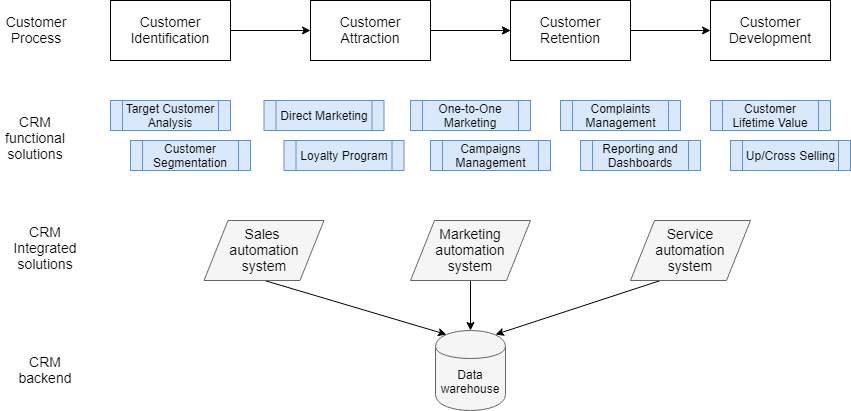
\includegraphics[width=12cm]{images/CRM-CustomerLifeCycle.png}
    \caption[CRM supports the customer life cycle]{CRM supports the customer life cycle. From \cite{DataAnalyticsinCRMProcessesALiteratureReview}}
    \label{fig:crm-clc}
\end{figure}

% How it does it
CRM systems are usually organized around four axes: Sales, Marketing, Support and Analysis\cite{crm-def}. The first three concern the operational part of a CRM, used for lead generation and conversion for example. An analytical part of the CRM takes care to analyze and generate insights from the data generated and collected by the operational processes. Through the years, CRM systems produce and store more and more data and \textit{Big data} techniques are needed used to make use of them, instead of just having them stored\cite{peel-et-al}.


% -------------------------------- Section: Why AI within CRM
\section{CRM AI}

CRM AI is a term that can be found in the litterature. But what does it really means ? Is it more than just a buzzword ? This section outlines the motivation and questions arising when combining CRM + AI.

This section details the motivations for combining CRM+AI and the resulting questions and interrogations.

\subsection{Artificial Intelligence within CRM}

Often cited as the next major vague of innovaiton, Artificial Intelligence (AI) can be the tool to optimize customer interactions based on the amount of data companies have. In its \textit{IT Glossary}\footnote{\url{https://www.gartner.com/it-glossary/artificial-intelligence/}}, Gartner defines AI as a technology that appears to emulate human performance. AI learns, comes to its own conclusion, appears to understand complex content, can engage into a natural dialogue with people, enhances human cognitive performance or replaces people in the execution of nonroutine tasks.

In a customer relationship management context, artificial intelligence can be used to enhance the current functionalities of CRMs. AI relies on data and for a company, all its customer-related data are stored in the CRM. By applying AI technologies into CRM applications like sales or service automation, current processes can evolve and new functionalities be created. AI has the ability to ingest data and assist CRM's user in their daily tasks, whether by intelligently analyzing a large volume of data or by being proactive and anticipating needs. The aim is to create more personalized customer experiences with findings uncovered by AI techniques and make a business \textit{smarter}


\subsection{Outline of the analysis}
% -------- Goal of the analysis
One of the aims of this thesis is to provided an overview of the integration of artificial intelligence technologies in a CRM context. With the advent of artificial intelligence and its relative ease of access, CRM vendors can consider a new product line around AI. When a CRM editor announces that it will soon integrate some AI components in its solutions, it aims to attract new customers while showing current customers that its system is innovative and at the cutting edge of technology.

CRM vendors claim to have easy to use and well integrated AI solutions, but what is really happening in those solutions? What are the kind of AI technologies used? How easy to configure are those AI features? Are they really useful for the business and tailored? All companies are different, but can they adapt these innovative solutions to their unique business? The research of this section tries to address those issues and really understand what is meant by \textit{CRM AI}.


% -------------------------------- Section: Editors Market
\section{Editors Market}


\subsection{CRM Editors analyzed}
% Ways of work


\subsection{CRM Editors review}
CRM Editors organized by alphabetical order ?

% -------------------------------- Section: DMP Platforms
\section{Data Management Platforms}
May be just a subsection, very fast on the subject


% -------------------------------- Section: Editors Ranking
\section{CRM Editors Ranking}


\subsection{Current state}


\subsection{Near feature status}


% -------------------------------- Section: Conclusion
\section{Conclusion}

Gartner:

    - CRM editors are leveraging AI capabilities such as machine learning and NLP to augment their application functionality. The current work made by the CRM editors concern embedded AI.
    - The advantage for a company to use such embedded AI is the ability to use a powerful emerging technology quickly, without a lot of investments. 
    - This is the premise of using AI in CRM.
    - In the market, CRM editors are using AI as an umbrella term to encompass a wide array of functionality, including machine learning (ML) powered data predictions and natural-language processing (NLP) pseudohuman interactions (e.g. chatbots).  CRM editors are integrating such new functionalities within their applications to enhance their CRM functionality.


    - The integrated CRM AI capabilities offered by enterprise vendors provide a path to learn and experiment with ML and NLP services without needing deep AI-based technical skills.
    - Current embedded AI offerings apply advance data-driven predictive capabilities to optimize customer-related decisions against narrow CRM functional use-cases.
    - CRM Editors will continue to invest in incremental improvements. This will lead to increased customization, configuration, and transparency into the underlying technical execution process of their embedded AI capabilities.
    - Using AI CRM functionality will not make CRM users data scientist. However, packaged CRM AI capabilities provide a path tho learn and experiment ML and NLP technologies directly with real-world data.
    - Create more differentiated solutions by integrating custom-defined ML models into your CRM applications once you have identified the unique data patterns and possible insights that embedded fucntionality has not.
    - Black box implementations. API acess to pretrained AI.
    
